\documentclass[10pt,twocolumn,letterpaper]{article}

\usepackage{cvpr}
\usepackage{times}
\usepackage{epsfig}
\usepackage{graphicx}
\usepackage{amsmath}
\usepackage{amssymb}
\usepackage{multirow}
\usepackage{caption}
\usepackage{subcaption}

% Include other packages here, before hyperref.

% If you comment hyperref and then uncomment it, you should delete
% egpaper.aux before re-running latex.  (Or just hit 'q' on the first latex
% run, let it finish, and you should be clear).
\usepackage[breaklinks=true,bookmarks=false]{hyperref}

\cvprfinalcopy % *** Uncomment this line for the final submission

\def\cvprPaperID{****} % *** Enter the CVPR Paper ID here
\def\httilde{\mbox{\tt\raisebox{-.5ex}{\symbol{126}}}}

% Pages are numbered in submission mode, and unnumbered in camera-ready
%\ifcvprfinal\pagestyle{empty}\fi
\setcounter{page}{1}
\graphicspath{{./figures/}}
\begin{document}

%%%%%%%%% TITLE
\title{Fast multi-object tracking by detection}

\author{Suraj M S\\
Georgia Institute of Technology\\
{\tt\small mssuraj@gatech.edu}
% For a paper whose authors are all at the same institution,
% omit the following lines up until the closing ``}''.
% Additional authors and addresses can be added with ``\and'',
% just like the second author.
% To save space, use either the email address or home page, not both
\and
Takuma Nakamura\\
Georgia Institute of Technology\\
{\tt\small takuma.nakamura@gatech.edu}
}

\maketitle
%\thispagestyle{empty}

%%%%%%%%% ABSTRACT
\begin{abstract}
   Object detection and tracking is a crucial part of computer vision systems with wide applications in autonomous navigation, surveillance, augmented reality, and video editing. Most of these applications require systems that are fast and accurate enough to be used in real-time settings.\\
	Recently, many convolutional neural network (CNN) models for fast object detection have emerged. We explore these models and ways to extend them for multi-object tracking whilst retaining their accuracy and speed.
\end{abstract}

%%%%%%%%% BODY TEXT
\section{Introduction}

Multi-object tracking is a fundamental problem in computer vision. However, the current state-of-the-art is far from human level performance and there is considerable room for improvement. Tracking-by-detection is one of the many methods used for this purpose. With the recent progress in real-time object detection models using CNNs, it is tempting to explore how we can exploit the temporal dependencies within the object detections in frames. We aim to build a system that retains the high accuracy and speed of these detection systems.\\

%-------------------------------------------------------------------------
%\section{Related work}
%\subsection{Object detection}
%\subsection{Object tracking}

\section{Baseline tests}
As a starting point, we decided to choose amongst the current state-of-the-art fast object detectors. Note that our criteria for these detectors are as follows:
\begin{itemize}
	\item have a reported implementation that runs on a Titan X GPU at a frame-rate of at least 5 frames per second
	\item have a reported mAP on the VOC2007\cite{everingham2010pascal} dataset above 70\%
\end{itemize}
We found the following detectors that satisfy this criteria:
\begin{center}
    \begin{tabular}{ | l | l | p{2cm}|}
    \hline
    Detector & FPS(Titan X) & mAP(\%)\\ 
    \hline
    Faster R-CNN\cite{DBLP:journals/corr/RenHG015} & 7 & 73.2\\
    YOLOv2\cite{DBLP:journals/corr/RedmonF16} & \textbf{67} & 76.8\\
    YOLOv2 544x544\cite{DBLP:journals/corr/RedmonF16} & 40 & 78.6\\
    SSD300\cite{liu2016ssd} & 46 & 77.2\\
    SSD512\cite{liu2016ssd} & 19 & \textbf{79.8}\\
    \hline
    \end{tabular}
\end{center}
Given the relatively slow frame-rate of Faster R-CNN without any substantial mAP improvement over the other detectors, we discard it.\\
Both YOLO and SSD have comparable frame-rate and mAP. Hence, we compare their performances to a new dataset.
\subsection{Dataset}
We choose the MOT16\cite{MOT16} dataset for this purpose since it has a variety of challenging sequences and also provides us a standardized benchmark for both detection and tracking tasks.\\
The MOT16 dataset contains 14 video sequences (7 training, 7 test) in unconstrained environments filmed with both static and moving cameras. We use only the training set for performing our tests since the ground truth annotations for them are openly available. The annotations are also accompanied by detections with the Deformable part models (DPM)\cite{felzenszwalb2010object}.\\
The training set consists of the following sequences:
\begin{center}
	\scalebox{0.9}{
	    \begin{tabular}{ | l | l | p{4cm}|}
	    \hline
	    Name & Frame count & Description\\ 
	    \hline
	    MOT16-02 & 600 & People walking around a large square\\
	    MOT16-04 & 1050 & Pedestrian street at night, elevated viewpoint\\
	    MOT16-05 & 837 & Street scene from a moving platform\\
	    MOT16-09 & 525 & A pedestrian street scene filmed from a low angle\\
    		MOT16-10 & 654 & A pedestrian scene filmed at night by a moving camera\\
	    MOT16-11 & 900 & Forward moving camera in a busy shopping mall\\
    		MOT16-13 & 750 & Filmed from a bus on a busy intersection\\
	    \hline
    		\end{tabular}
    }
\end{center}

\subsection{YOLOv2 }
We decided to use YOLOv2 416×416 which is available off-the-shelf at \url{https://pjreddie.com/darknet/yolo/}. We tested the CPU implementation of this detector only with the MOT16-02 sequence due to hardware and time constraints - this let us compare it against our measurements on SSD which were performed only with a CPU implementation. \\
We decided to switch to the GPU implementation for measuring the accuracy performance.


\subsection{SSD300}
We chose SSD300 since it is faster than its 512 counterpart and also available off-the-shelf at \url{https://github.com/weiliu89/caffe/tree/ssd}.
We tested the CPU implementation with the entire MOT16 training dataset. We could not run the GPU implementation yet. We plan to do so next week.

\subsection{Testing hardware}
We used an Intel(R) Core(TM) i7-6500U CPU @ 2.50GHz with 12 GB RAM running (Arch)Linux kernel 4.10.2 for testing SSD and YOLO (CPU mode). For the YOLO GPU mode tests, we used an Intel(R) Core(TM) i7-6820 CPU @ 2.7GHz with an nVidia GTX980 GPU.

\subsection{YOLO vs SSD}
\subsubsection*{Quantitative analysis}
\begin{center}
    \begin{tabular}{ | l | l | l | l | l | l |}
    \hline
    Dataset & \multicolumn{2}{|c|}{Time/frame (sec)} & \multicolumn{3}{|c|}{Average Precision (\%)}\\
    \cline{2-6}
     & YOLO & SSD & YOLO & SSD & DPM\\
    \hline
    MOT16-02 & 7.57145 & 1.36 & 25 & 35 & 56\\
    MOT16-04 & - & 1.27 & 11 & 36 & 68\\
    MOT16-05 & - & 1.43 & 59 & 61 & 56\\
    MOT16-09 & - & 1.37 & 58 & 75 & 76\\
    MOT16-10 & - & 1.26 & 07 & 35 & 52\\
    MOT16-11 & - & 1.26 & 59 & 62 & 77\\
    MOT16-13 & - & 1.25 & 00 & 05 & 33\\
    \hline
    \end{tabular}
\end{center}
In terms of speed, SSD outperforms YOLO by a significant margin (approximately 5.5 times faster). Perhaps, this margin will not be so drastic when both are tested on a GPU. We plan to run the SSD tests on a GPU system next week.\\
In terms of precision, again SSD performs better than YOLO on all the sequences.

\subsubsection*{Qualitative analysis}
We find that both SSD and YOLO fail badly with distant objects and also when the camera viewpoint is at a high angle. In addition, on many occasions they fail when there are dense multiple instances of an object (eg. pedestrians in a crowded scene). However, in general, SSD seems to generate more accurate detections than YOLO. \\
Since most of the object instances are pedestrians, DPM performs better than SSD and YOLO. This can be rectified by fine-tuning our detector with pedestrian heavy dataset such as MOT16.\\

\begin{figure}[!tbp]
  \begin{subfigure}[b]{0.3\textwidth}
    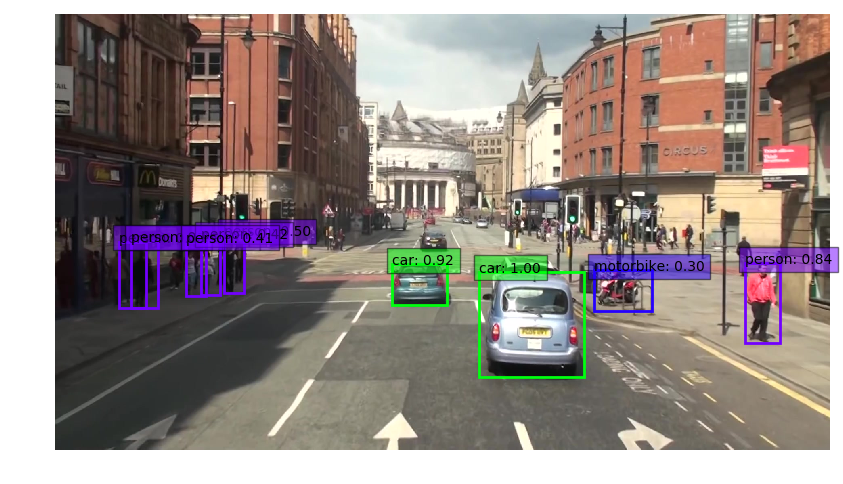
\includegraphics[width=\textwidth]{ssd_mot16-13-100.png}
    \caption{SSD}
    \label{fig:ssd_mot16_13_100}
  \end{subfigure}
  \hfill
  \begin{subfigure}[b]{0.3\textwidth}
    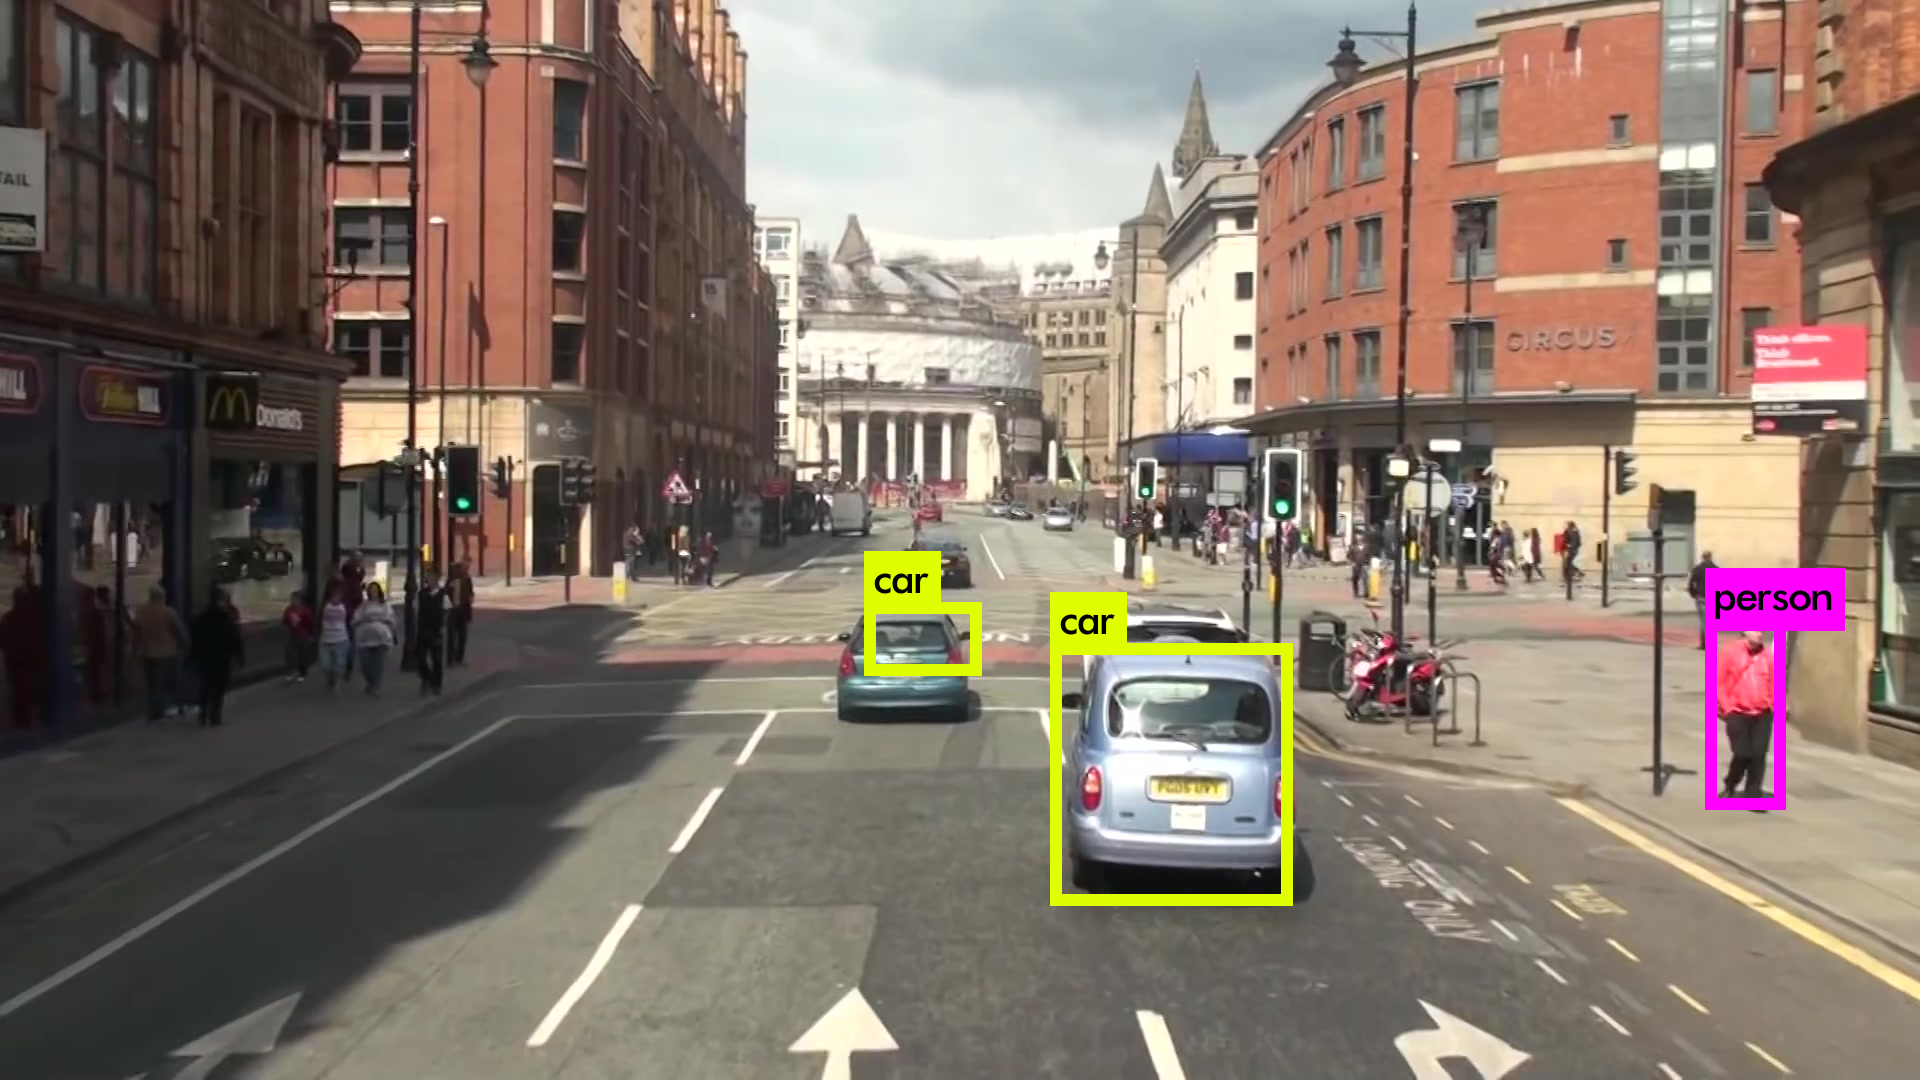
\includegraphics[width=\textwidth]{yolo_mot16-13-100.png}
    \caption{YOLO}
    \label{fig:yolo_mot16_13_100}
  \end{subfigure}
  \begin{subfigure}[b]{0.3\textwidth}
    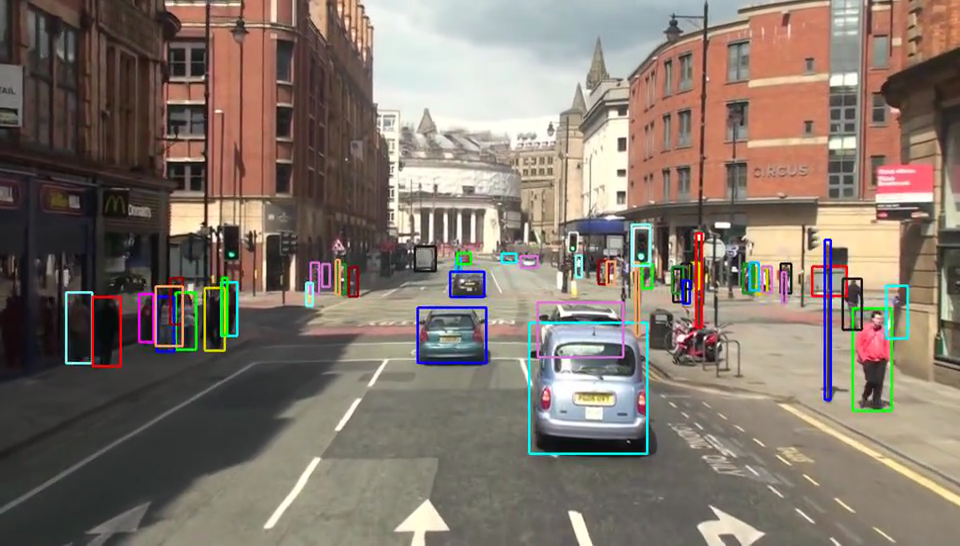
\includegraphics[width=\textwidth]{gt_mot16-13-100.png}
    \caption{Ground truth}
    \label{fig:yolo_mot16_13_100}
  \end{subfigure}
  \caption{Detections on frame 100 in MOT16-13}
\end{figure}

\section{Next steps}
Given the results we have, we will most likely proceed with SSD as our base detector model. We plan to investigate the following tracking models:
\begin{itemize}
	\item Detector model $\rightarrow$ [detections] $\rightarrow$ simple off-the-shelf post-process tracker $\rightarrow$ [tracks] (our baseline model)
	\item Detector model $\rightarrow$ [detections] $\rightarrow$ siamese/triplet loss network on consecutive frames $\rightarrow$ [tracks]	
	\item Detector model $\rightarrow$ [detections] $\rightarrow$ RNN based post process tracker $\rightarrow$ simple post-processing $\rightarrow$ [tracks]
	\item We use multiple layers from the detector model and augment it with other layers to create an end-to-end trainable network. Essentially, we use the trained detector as a good initialization for the sub-segment corresponding to the original detector layers in our new model.
\end{itemize}

{\small
\bibliographystyle{ieee}
\bibliography{egbib}
}

\end{document}
